\documentclass{beamer}

\usepackage{layout}

\title{Recap}
\subtitle{Week 3}
\author{Mario Supersaxo \\ Daniel Winz \\ Marc Nyffenegger}

\begin{document}

\maketitle


\section*{Programm}
\begin{frame}
\tableofcontents
\end{frame}

\section{Slide-Grundlagen}

\subsection{Blöcke}

%%%%% ein Slide
\begin{frame}
	\frametitle{Blöcke \hfill \footnotesize{Hochschule Luzern}}
	\framesubtitle{Standardblöcke im Vergleich \hfill \tiny{Technik \& Architektur}}
	
	\begin{block}{Regulärer Block}
		Das ist ein regulärer Block.
	\end{block}

	\begin{alertblock}{Alarmblock}
		Das ist ein Alarmblock.
	\end{alertblock}

	\begin{exampleblock}{Beispielblock}
		Das ist ein Beispielblock.
	\end{exampleblock}
\end{frame}

\subsection{Kolonnen}

\begin{frame}
	\frametitle{Slides splaten \hfill \footnotesize{Hochschule Luzern}}
	\framesubtitle{Vertikale Trennung \hfill \tiny{Technik \& Architektur}}

	\begin{columns}
		\begin{column}{5cm}
			\begin{block}{Links}
				Linke Kolonne
			\end{block}
		\end{column}
		\begin{column}{5cm}
			\begin{block}{Rechts}
				Rechte Kolonne
			\end{block}
		\end{column}
	\end{columns}
\end{frame}

\section{Syncronization}
\subsection{Why synchronization}
\begin{frame}
    \frametitle{Why synchronization?}
%    \framesubtitle{Framesubtitle}
    Computer operates in different time scale
    \begin{itemize}
        \item if slower than reality: Result too late $\Rightarrow$ INCORRECT
        \item if faster than reality: Result too early $\Rightarrow$ INCORRECT
    \end{itemize}
    Computer has to synchronize with process
    \begin{figure}
        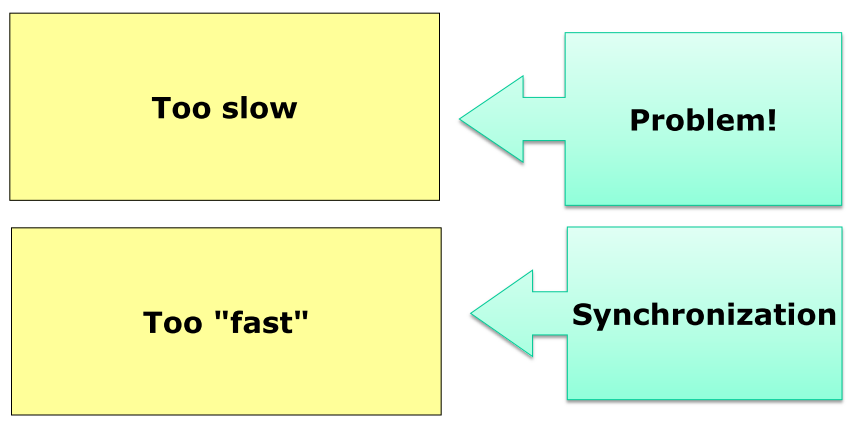
\includegraphics[width=0.5\textwidth]{fig/synchronization.png}
        \caption{Synchronization}
    \end{figure}
\end{frame}

\subsection{Realtime Synchronization}
\begin{frame}
    \frametitle{Realtime Synchronization}
%    \framesubtitle{Anotherframesubtitle}
    \begin{figure}
        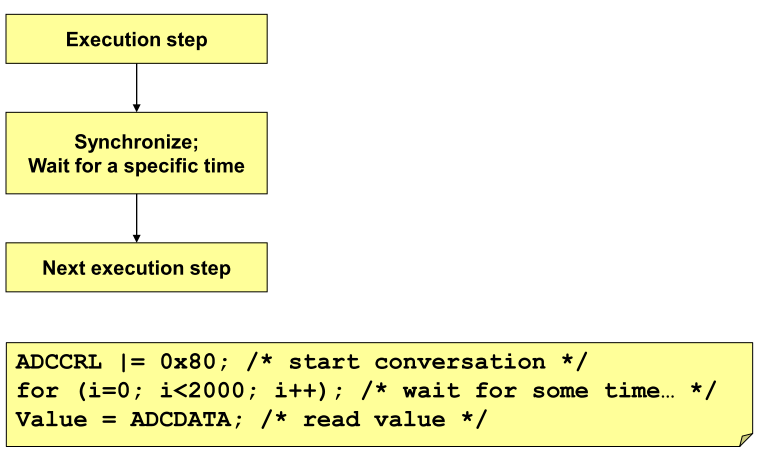
\includegraphics[width=0.7\textwidth]{fig/realtime.png}
        \caption{Realtime Synchronization}
    \end{figure}
\end{frame}

\begin{frame}
    \frametitle{Realtime Synchronization}
%    \framesubtitle{Anotherframesubtitle}
        \begin{exampleblock}{+}
        \begin{itemize}
			\item easy to implement         
    	\end{itemize}
    \end{exampleblock}
    \begin{alertblock}{-}
        \begin{itemize}
			\item Inefficient        
        	\item Needed waiting time?
        	\item Different Compiler
        	\item Different clock rate
    	\end{itemize}
    \end{alertblock}
\end{frame}

\subsection{Gadfly Synchronization}
\begin{frame}
    \frametitle{Gadfly Synchronization}
%    \framesubtitle{Anotherframesubtitle}
    \begin{figure}
        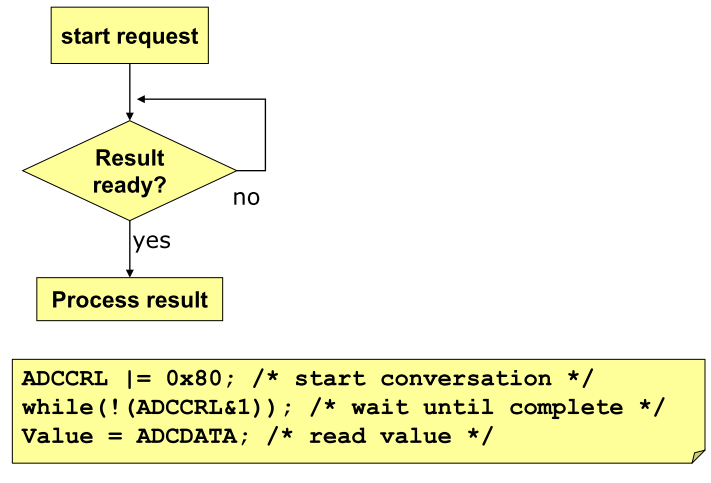
\includegraphics[width=0.7\textwidth]{fig/gadfly.png}
        \caption{Gadfly Synchronization}
    \end{figure}
        
\end{frame}

\begin{frame}
    \frametitle{Gadfly Synchronization}
%    \framesubtitle{Anotherframesubtitle}
	\begin{exampleblock}{+}
        \begin{itemize}
			\item easy to implement
			\item lowers the system latency (reading data when it is available)         
    	\end{itemize}
   	\end{exampleblock}	
	\begin{alertblock}{-}    
    	\begin{itemize}
			\item Active waiting/polling (Flags)
			\item Processing power needed 
			\item Blocks further execution 
	     \end{itemize}
	\end{alertblock}   
\end{frame}

\subsection{Interrupt Synchronization}
\begin{frame}
    \frametitle{Interrupt Synchronization}
%    \framesubtitle{Anotherframesubtitle}
    \begin{figure}
        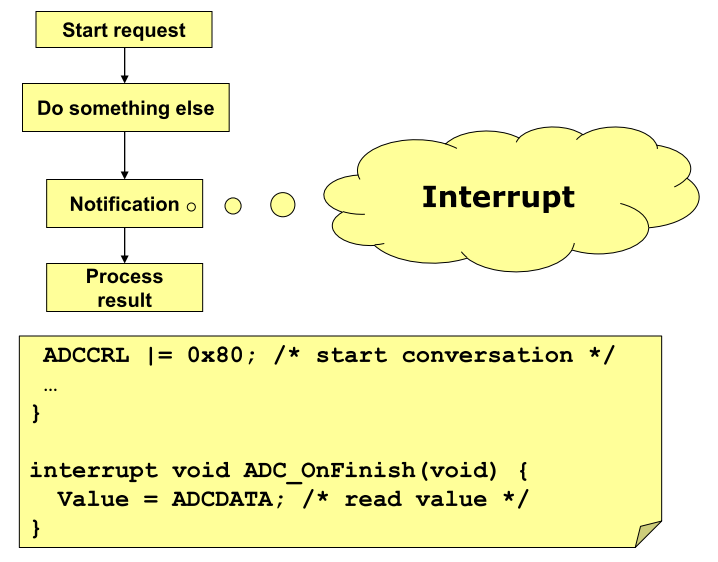
\includegraphics[width=0.6\textwidth]{fig/interrupt.png}
        \caption{Interrupt Synchronization}
    \end{figure}
        
\end{frame}

\begin{frame}
    \frametitle{Interrupt Synchronization}
 %   \framesubtitle{Anotherframesubtitle}
	\begin{exampleblock}{+}
        \begin{itemize}
			\item No waiting
			\item Better Performance (consider overhead)         
    	\end{itemize}
   	\end{exampleblock}	
	\begin{alertblock}{-}    
    	\begin{itemize}
			\item Can easily get complicated
	     \end{itemize}
	\end{alertblock}
        
\end{frame}
\section{Interrupts}
\subsection*{What is an interrupt? }
\begin{frame}
    \frametitle{What is an Interrupt? }
    \begin{figure}
        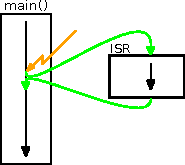
\includegraphics[height=0.4\textheight]{fig/interrupt.pdf}
        \caption{Interrupt}
    \end{figure}
\end{frame}

\subsection*{Nested interrupts}
\begin{frame}
    \frametitle{Nested interrupts}
    \begin{figure}
        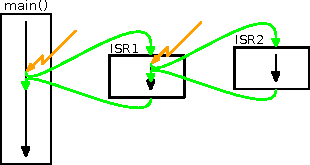
\includegraphics[height=0.4\textheight]{fig/interrupt_nested.pdf}
        \caption{nested interrupt}
    \end{figure}
\end{frame}

\subsection*{Reentrancy}
\begin{frame}
    \frametitle{Reentrancy}
    \begin{figure}
        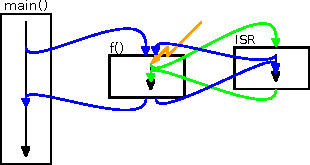
\includegraphics[height=0.4\textheight]{fig/interrupt_reentrancy.pdf}
        \caption{Non reentrant function f()}
    \end{figure}
\end{frame}


\section{ARM Cortex}
\subsection{Overview}
\begin{frame}
    \frametitle{ARM}
    \framesubtitle{Overview}
    ARM Cortex
    \begin{itemize}
        \item \textbf{A}dvanced \textbf{R}ISC \textbf{M}achines
        \item sell License
        \item up to 64bit
    \end{itemize}
    \begin{block}{ARM Today}
		The Apple A8 is built up of a 64-Bit-ARM-CPU
    \end{block}
\end{frame}

\subsection{Families}
\begin{frame}
    \frametitle{ARM}
    \framesubtitle{Families}
   ARM Cortex Families:
    \begin{itemize}
        \item A: Application
        \item R: Realtime
        \item \textbf{M: Microcontroller}
    \end{itemize}
    \begin{block}{Instruction Set}
        M0,\textbf{ M0+}, M1 <  M3 <  \textbf{M4} < M4 FPU
    \end{block}
\end{frame}

\subsection{Instruction set}
\begin{frame}
    \frametitle{ARM}
    \framesubtitle{Instruction set}
    \begin{figure}
        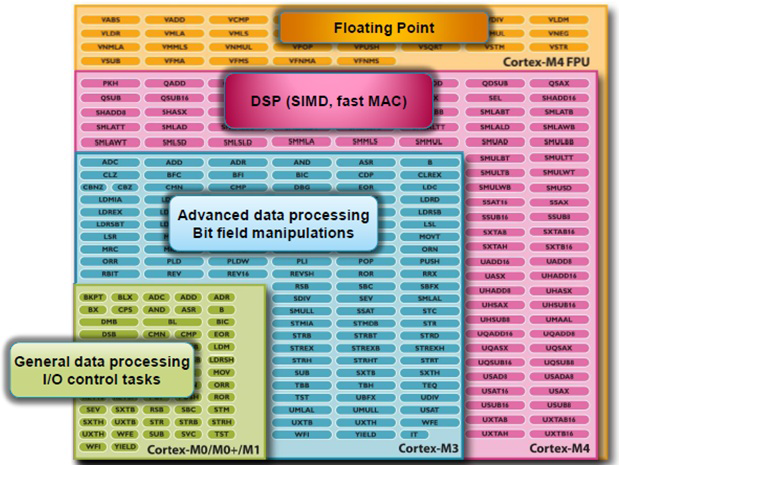
\includegraphics[width=0.8\textwidth]			{fig/instructionset.png}
        \caption{Instruction set}
    \end{figure}
\end{frame}

\subsection{Interrupts}
\begin{frame}
    \frametitle{ARM}
    \framesubtitle{Interrupts}
    16 predefined Interrupts
    Priorities
        \begin{itemize}
        \item 8bit Priority Register
        \item FSL M0+: 2bits = 4 Priorities
        \item FSL M4 : 4bits = 16 Prio
    \end{itemize}
    \begin{block}{Reihenfolge Priorities}
        the lower the prio or subprio number - the higher prio!
    \end{block}
\end{frame}


\end{document}
